%=========================================================================
% (c) 2011, 2012 Josef Lusticky <xlusti00@stud.fit.vutbr.cz>

\chapter{Network Time Protocol}
Network Time Protocol provides mechanism for synchronising systems' clocks over the variable-latency data network.
NTP was introduced and is still developed by David Mills at University of Delaware in Newark, United States.
NTP is argueably the longest running, continuously operating,
ubiquitously available protocol in the Internet~\cite{ntp-overview}.
Despite being one of the oldest surviving protocol on the Internet it is not old-fashioned at all.
NTP version 4 described in RFC~5905~\cite{rfc5905} is an update to older NTPv3 to accomodate NTP to IPv6.
Version 4 also includes improvements in
the mitigation and discipline algorithms that extend
the potential accuracy to the tens of microseconds with modern
workstations and fast LANs~\cite{rfc5905}.
NTPv4 corrects some
errors in NTPv3 design and includes optional extension mechanism
that can be used for adding more capabilites to NTP, e.g. the
Autokey security protocol described in RFC~5906~\cite{rfc5906}
for authenticating servers to clients.

Simple Network Time Protocol is simplified NTP implementation lacking complex
synchronisation algorithms used by NTP.
SNTP is also described in RFC 5906~\cite{rfc5906}.
\!...
SNTP is a simplified sub-set of the algorithms used by the NTP protocol.

NTP always uses the Coordinated Universal Time.
NTP manipulates with the time through timestamps - a record of time.
NTP timestamp has two parts - part for expressing the number of seconds
and part for fraction of a second. \!Called RFC
It has never been a goal of NTP to take care of local time,
it is up to operating system to provide user the correct local time~\cite{ntp-overview}.

\section{Topology and Hierarchy}
As in every other network protocol there are servers and clients in NTP.
The servers are rated with the stratum (plural form strata) number which represents their position
in an NTP hierarchy and their possible accurancy.
Primary (stratum 1) servers synchronise to the reference clock directly traceable to UTC via
radio, satellite or modem.
The stratum 2 servers synchronise to stratum 1
servers via hierarchical subnet.
The stratum 3 servers synchronise to stratum 2 servers, and so on.

\begin{figure}
  \centering
  %\input{./xfig/test.pstex_t}
  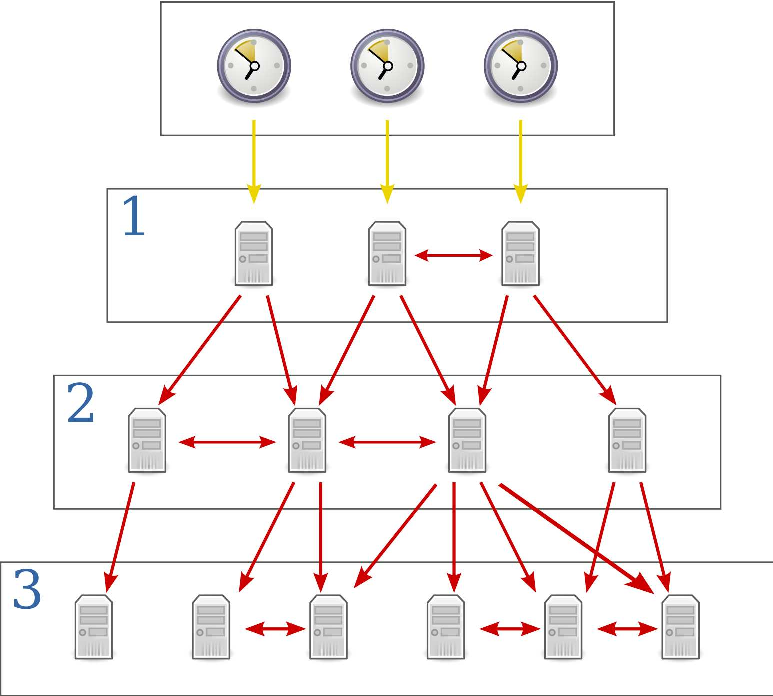
\includegraphics[width=10cm,keepaspectratio]{fig/Network_Time_Protocol_servers_and_clients.pdf}
  \caption{Topology and Hierarchy of NTP}
  \label{fig:ntp-hierarchy}
\end{figure}


\! 
\! rfc5905
\! older "Time" protocol


\section{Time and timestamps}
\!WHAT IS UTC - definition
The time specified by UTC is the same for all timezones.
%The Coordinated Universal Time (UTC) timescale represents mean solar
%time as disseminated by national standards laboratories.
The system time is represented by the system clock maintained by
the hardware and operating system.
The goal of the NTP algorithms is to minimize
both the time difference and frequency difference between UTC and the system clock.
When these differences have been reduced below nominal
tolerances, the system clock is said to be synchronised to UTC.

\section{Network}\label{sec:ntp-network}
Network specification of NTP 
The protocol uses the User Datagram Protocol (UDP) on port number 123~\cite{ianna-ports}.
The NTP packet is a UDP datagram, carried on port 123.

\subsection{Packet structure}
The 64-bit timestamps used by NTP consist of a 32-bit seconds part and a 32-bit fractional second part.

\section{Algorithms}

\section{Errors}
Jitter, ....
